% Options for packages loaded elsewhere
\PassOptionsToPackage{unicode}{hyperref}
\PassOptionsToPackage{hyphens}{url}
%
\documentclass[
  ignorenonframetext,
]{beamer}
\usepackage{pgfpages}
\setbeamertemplate{caption}[numbered]
\setbeamertemplate{caption label separator}{: }
\setbeamercolor{caption name}{fg=normal text.fg}
\beamertemplatenavigationsymbolsempty
% Prevent slide breaks in the middle of a paragraph
\widowpenalties 1 10000
\raggedbottom
\setbeamertemplate{part page}{
  \centering
  \begin{beamercolorbox}[sep=16pt,center]{part title}
    \usebeamerfont{part title}\insertpart\par
  \end{beamercolorbox}
}
\setbeamertemplate{section page}{
  \centering
  \begin{beamercolorbox}[sep=12pt,center]{part title}
    \usebeamerfont{section title}\insertsection\par
  \end{beamercolorbox}
}
\setbeamertemplate{subsection page}{
  \centering
  \begin{beamercolorbox}[sep=8pt,center]{part title}
    \usebeamerfont{subsection title}\insertsubsection\par
  \end{beamercolorbox}
}
\AtBeginPart{
  \frame{\partpage}
}
\AtBeginSection{
  \ifbibliography
  \else
    \frame{\sectionpage}
  \fi
}
\AtBeginSubsection{
  \frame{\subsectionpage}
}
\usepackage{amsmath,amssymb}
\usepackage{lmodern}
\usepackage{iftex}
\ifPDFTeX
  \usepackage[T1]{fontenc}
  \usepackage[utf8]{inputenc}
  \usepackage{textcomp} % provide euro and other symbols
\else % if luatex or xetex
  \usepackage{unicode-math}
  \defaultfontfeatures{Scale=MatchLowercase}
  \defaultfontfeatures[\rmfamily]{Ligatures=TeX,Scale=1}
\fi
% Use upquote if available, for straight quotes in verbatim environments
\IfFileExists{upquote.sty}{\usepackage{upquote}}{}
\IfFileExists{microtype.sty}{% use microtype if available
  \usepackage[]{microtype}
  \UseMicrotypeSet[protrusion]{basicmath} % disable protrusion for tt fonts
}{}
\makeatletter
\@ifundefined{KOMAClassName}{% if non-KOMA class
  \IfFileExists{parskip.sty}{%
    \usepackage{parskip}
  }{% else
    \setlength{\parindent}{0pt}
    \setlength{\parskip}{6pt plus 2pt minus 1pt}}
}{% if KOMA class
  \KOMAoptions{parskip=half}}
\makeatother
\usepackage{xcolor}
\IfFileExists{xurl.sty}{\usepackage{xurl}}{} % add URL line breaks if available
\IfFileExists{bookmark.sty}{\usepackage{bookmark}}{\usepackage{hyperref}}
\hypersetup{
  pdftitle={Why Do RSL Fans Cheer Longer Than Jazz Fans?},
  pdfauthor={Tom Coe, Joey Brignone, Darren Rou},
  hidelinks,
  pdfcreator={LaTeX via pandoc}}
\urlstyle{same} % disable monospaced font for URLs
\newif\ifbibliography
\usepackage{color}
\usepackage{fancyvrb}
\newcommand{\VerbBar}{|}
\newcommand{\VERB}{\Verb[commandchars=\\\{\}]}
\DefineVerbatimEnvironment{Highlighting}{Verbatim}{commandchars=\\\{\}}
% Add ',fontsize=\small' for more characters per line
\usepackage{framed}
\definecolor{shadecolor}{RGB}{248,248,248}
\newenvironment{Shaded}{\begin{snugshade}}{\end{snugshade}}
\newcommand{\AlertTok}[1]{\textcolor[rgb]{0.94,0.16,0.16}{#1}}
\newcommand{\AnnotationTok}[1]{\textcolor[rgb]{0.56,0.35,0.01}{\textbf{\textit{#1}}}}
\newcommand{\AttributeTok}[1]{\textcolor[rgb]{0.77,0.63,0.00}{#1}}
\newcommand{\BaseNTok}[1]{\textcolor[rgb]{0.00,0.00,0.81}{#1}}
\newcommand{\BuiltInTok}[1]{#1}
\newcommand{\CharTok}[1]{\textcolor[rgb]{0.31,0.60,0.02}{#1}}
\newcommand{\CommentTok}[1]{\textcolor[rgb]{0.56,0.35,0.01}{\textit{#1}}}
\newcommand{\CommentVarTok}[1]{\textcolor[rgb]{0.56,0.35,0.01}{\textbf{\textit{#1}}}}
\newcommand{\ConstantTok}[1]{\textcolor[rgb]{0.00,0.00,0.00}{#1}}
\newcommand{\ControlFlowTok}[1]{\textcolor[rgb]{0.13,0.29,0.53}{\textbf{#1}}}
\newcommand{\DataTypeTok}[1]{\textcolor[rgb]{0.13,0.29,0.53}{#1}}
\newcommand{\DecValTok}[1]{\textcolor[rgb]{0.00,0.00,0.81}{#1}}
\newcommand{\DocumentationTok}[1]{\textcolor[rgb]{0.56,0.35,0.01}{\textbf{\textit{#1}}}}
\newcommand{\ErrorTok}[1]{\textcolor[rgb]{0.64,0.00,0.00}{\textbf{#1}}}
\newcommand{\ExtensionTok}[1]{#1}
\newcommand{\FloatTok}[1]{\textcolor[rgb]{0.00,0.00,0.81}{#1}}
\newcommand{\FunctionTok}[1]{\textcolor[rgb]{0.00,0.00,0.00}{#1}}
\newcommand{\ImportTok}[1]{#1}
\newcommand{\InformationTok}[1]{\textcolor[rgb]{0.56,0.35,0.01}{\textbf{\textit{#1}}}}
\newcommand{\KeywordTok}[1]{\textcolor[rgb]{0.13,0.29,0.53}{\textbf{#1}}}
\newcommand{\NormalTok}[1]{#1}
\newcommand{\OperatorTok}[1]{\textcolor[rgb]{0.81,0.36,0.00}{\textbf{#1}}}
\newcommand{\OtherTok}[1]{\textcolor[rgb]{0.56,0.35,0.01}{#1}}
\newcommand{\PreprocessorTok}[1]{\textcolor[rgb]{0.56,0.35,0.01}{\textit{#1}}}
\newcommand{\RegionMarkerTok}[1]{#1}
\newcommand{\SpecialCharTok}[1]{\textcolor[rgb]{0.00,0.00,0.00}{#1}}
\newcommand{\SpecialStringTok}[1]{\textcolor[rgb]{0.31,0.60,0.02}{#1}}
\newcommand{\StringTok}[1]{\textcolor[rgb]{0.31,0.60,0.02}{#1}}
\newcommand{\VariableTok}[1]{\textcolor[rgb]{0.00,0.00,0.00}{#1}}
\newcommand{\VerbatimStringTok}[1]{\textcolor[rgb]{0.31,0.60,0.02}{#1}}
\newcommand{\WarningTok}[1]{\textcolor[rgb]{0.56,0.35,0.01}{\textbf{\textit{#1}}}}
\usepackage{graphicx}
\makeatletter
\def\maxwidth{\ifdim\Gin@nat@width>\linewidth\linewidth\else\Gin@nat@width\fi}
\def\maxheight{\ifdim\Gin@nat@height>\textheight\textheight\else\Gin@nat@height\fi}
\makeatother
% Scale images if necessary, so that they will not overflow the page
% margins by default, and it is still possible to overwrite the defaults
% using explicit options in \includegraphics[width, height, ...]{}
\setkeys{Gin}{width=\maxwidth,height=\maxheight,keepaspectratio}
% Set default figure placement to htbp
\makeatletter
\def\fps@figure{htbp}
\makeatother
\setlength{\emergencystretch}{3em} % prevent overfull lines
\providecommand{\tightlist}{%
  \setlength{\itemsep}{0pt}\setlength{\parskip}{0pt}}
\setcounter{secnumdepth}{-\maxdimen} % remove section numbering
\ifLuaTeX
  \usepackage{selnolig}  % disable illegal ligatures
\fi

\title{Why Do RSL Fans Cheer Longer Than Jazz Fans?}
\author{Tom Coe, Joey Brignone, Darren Rou}
\date{April 29, 2022}

\begin{document}
\frame{\titlepage}

\begin{frame}{Introduction}
\protect\hypertarget{introduction}{}
If you've ever been to a MLS game you know the crowd goes crazy when
their team scores a goal. In comparison at an NBA game the crowd cheers,
but without the same amount of enthusiasm. This study aims to look into
this phenomenon and see if we can find important factors that contribute
to this. The hypothesis of this study is that the amount of time a crowd
cheers is dependent on the number of points scored per game. To
investigate this question we will look at Utah's professional soccer and
basketball teams Real Salt Lake (RSL) and the Utah Jazz. First we will
collect data on the total points scored for these teams. Then, we will
collect data on how long each team's respective crowd cheers when they
score a point. We will then compare these values and see if there is any
connection between them.
\end{frame}

\begin{frame}{Data Discovery}
\protect\hypertarget{data-discovery}{}
\begin{block}{Scoring Data}
\protect\hypertarget{scoring-data}{}
\href{https://www.nba.com/stats/teams/boxscores/?Season=2020-21\&SeasonType=Regular\%20Season\&CF=TEAM_NAME*E*Utah\%20Jazz}{nba.com}
provides scoring data for NBA teams. This website allows filtering of
data by team, season, and the type of game (regular, playoffs, etc.). We
note that there aren't many playoff games for the Jazz. With this taken
into consideration, we choose to take all scoring data from playoff,
play-in, and regular season games. We do so with the assumption that
games scores do not depend on the type of game. This assumption is
reasonable for our purposes. We are interested in the total points
scored by the Utah Jazz each game.

We repeat the same process of the RSL. We collect data about the total
points scored each game.
\end{block}

\begin{block}{Cheering Data}
\protect\hypertarget{cheering-data}{}
To collect data, we watched RSL and Jazz games and observed the crowd
when there was an instance of scoring. Then, using a stopwatch we timed
the duration of the crowd's cheering. For the basketball games this was
simple as there are no cuts in the video feed, but for soccer game this
was a little harder. Since there is a delay in game play after a goal is
scored in soccer the broadcasting network cuts away from the live feed
and shows instant replays. These replays, however, still have live audio
from the commentators and the crowd can still be heard. Thus, to gather
data for the celebration time we focused on listening to the crowd
during the replays and did our best to estimate when the crowd had
stopped cheering. The act of timing the crowd's reaction introduces
error in itself, but the added difficulty of not having a single
continuous video feed made accurate data collection even more difficult.
\end{block}
\end{frame}

\begin{frame}{Methodology}
\protect\hypertarget{methodology}{}
After data collection, we were given many measurements to choose from.
The first population sample we wish to evaluate will be the scores per
game. In order to adequately answer our question we will first analyze
how much one point in soccer is compared to one point in basketball. We
will need to take the scoring data collected and compare the means of
each data set. To do this we will assume these data sets follow a normal
distribution and will use t-tests to construct confidence intervals to
approximate the value of the population means. Since we are fairly
confident in our data, yet we recognize possible biases that are
present, we will be using a confidence interval of 95\%. Through this
t-test of 95\% confidence, we can find a range for the population mean
for the scores per game of RSL and of the Jazz.

Next, we wish to use this information to see why RSL fans cheer longer
than Jazz Fans. From our data sets, we will take the sample of cheer
time per point, plot a histogram and normal curve, and analyze our
results. This should prepare us to run another t-test of this sample, to
find a range wherein lies the population mean. For consistency, we will
use the 95\% confidence interval from before. Once both t-tests are run
for both cheer time data sets, we may start to draw conclusions from our
results.

One experimental parameter is this important is the sample size. It is
conventional to have a sample size of 30 or greater. We will consider
the t-scores which arises from using a sample size of 50. For sample
size of 50 and a 95\% confidence interval. The result is 2.0095752. This
is a good value for our experiment. This number means we have a 95\%
chance, that our sample mean will be within about 2 standard deviations
of the true population mean.

We will now consider what 2 t-scores means in terms of fans' celebration
time. We will use external knowledge of sports games. Using our
knowledge of sports games, we can say that the standard deviation of
fans' celebration times is probably much lower than 60 seconds. We will
use 60 seconds as the standard deviation as a worse case scenario. In
terms of a t-score of 2, we have an estimated EBM of

\[
2 \frac{60}{\sqrt{50}}
\]

which evaluates to 16.9705627. Considering that 60 is probably much
higher than the true value, this value is not bad. For example, if
instead the standard deviation was a more reasonable value, say, around
10, then we would have gotten 2.8284271 as our EBM.

In other words, in a bad case (standard deviation of around 60 seconds),
the width of our confidence interval will be about twice 16.9705627 or
about 34 seconds. In a good case (standard deviation of about 10
seconds), the width of our confidence interval will be about twice
2.8284271 or about 5.7 seconds. Considering all of this, we will decide
that a sample size of 50 (or greater) with our constructed 95\%
confidence interval is suitable for our experiment.
\end{frame}

\begin{frame}[fragile]{Analysis}
\protect\hypertarget{analysis}{}
\begin{block}{One Point In Soccer Is Worth X Points In Baseketball}
\protect\hypertarget{one-point-in-soccer-is-worth-x-points-in-baseketball}{}
We consider the total points scored by the Jazz each game in the
2019--2020 and 2020--2021 seasons. We put this data into a \texttt{.csv}
file, and using the \texttt{head()} function, we can create a table to
see what it looks like:

\begin{table}
\centering
\begin{tabular}{c|c|c|c|c|c}
\hline
Team & Match Up & Game Date & W/L & Min & Points\\
\hline
UTA & UTA @ LAC & 06/18/2021 & L & 240 & 119\\
\hline
UTA & UTA vs. LAC & 06/16/2021 & L & 240 & 111\\
\hline
UTA & UTA @ LAC & 06/14/2021 & L & 240 & 104\\
\hline
UTA & UTA @ LAC & 06/12/2021 & L & 240 & 106\\
\hline
UTA & UTA vs. LAC & 06/10/2021 & W & 240 & 117\\
\hline
UTA & UTA vs. LAC & 06/08/2021 & W & 240 & 112\\
\hline
\end{tabular}
\end{table}

As we can see, the \texttt{Points} column corresponds to total points
scored by the Jazz during a game.

The population we would like to consider consists of all points scored
by the Jazz in a game. Our sample (shown earlier) represents only a
small portion of the population, but it is sufficient for the motivation
for this study. We will now do some basic analysis on the data.

\begin{verbatim}
##    Min. 1st Qu.  Median    Mean 3rd Qu.    Max. 
##      78     106     114     114     122     154
\end{verbatim}

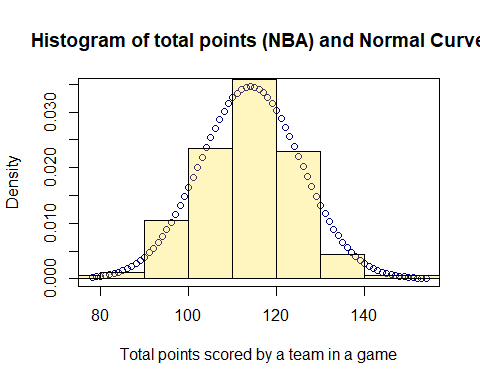
\includegraphics{finalpresentation_files/figure-beamer/unnamed-chunk-3-1.pdf}

The previous histogram had a sample size of 162. We find the sample mean
to be 114.0432099 and the sample standard deviation to be 11.5163124. As
shown by the previous histogram, the data is approximately normal, and
using a t-distribution for analysis is suitable.

\begin{verbatim}
## 
##  One Sample t-test
## 
## data:  nbaScores
## t = 126.04, df = 161, p-value < 2.2e-16
## alternative hypothesis: true mean is not equal to 0
## 95 percent confidence interval:
##  112.2564 115.8300
## sample estimates:
## mean of x 
##  114.0432
\end{verbatim}

The previous t-test gives a 95\% confidence interval of (112.2563898,
115.83003). In terms of NBA scores, this interval is quite small. Our
sample suggests the mean points scored by a team in an NBA points in
this interval with 95\% confidence.

Note that the data we obtained from nba.com is biased. We only sampled
from the 2020-2021 season, and we only sampled from playoff games. But
for our purposes, this biased sample should be sufficient.

Now, we consider data for the MLS. Similar to our NBA analysis, we want
to consider the total points scored by the RSL in a game.

\begin{table}
\centering
\begin{tabular}{c|c|c}
\hline
Team & Final Score & Year\\
\hline
RSL & 0 & 2022\\
\hline
RSL & 0 & 2022\\
\hline
RSL & 2 & 2022\\
\hline
RSL & 1 & 2022\\
\hline
RSL & 0 & 2022\\
\hline
RSL & 2 & 2022\\
\hline
\end{tabular}
\end{table}

Above is a table representing the data retrieved from kaggle.com. The
column we are interested in for our study's purposes is the
\texttt{Final\ Score}.

Similar to before, let \(Y\) be the total number of points scored by a
team in an MLS game.

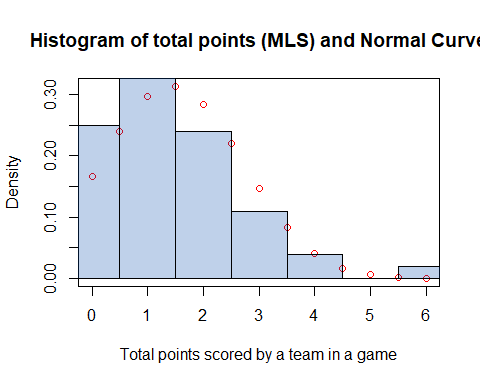
\includegraphics{finalpresentation_files/figure-beamer/unnamed-chunk-6-1.pdf}

The previous histogram had a sample size of 100. We find the sample mean
to be 1.43, and we find the sample standard deviation to be 1.2733079.
Compared to the sample mean, the sample standard deviation is quite
large. The previous histograms shows that RSL scores approximately
follow a normal distribution. Note that the data seems to be skewed
left. We can use a t-test to find a confidence interval.

\begin{verbatim}
## 
##  One Sample t-test
## 
## data:  mlsScores
## t = 11.231, df = 99, p-value < 2.2e-16
## alternative hypothesis: true mean is not equal to 0
## 95 percent confidence interval:
##  1.177348 1.682652
## sample estimates:
## mean of x 
##      1.43
\end{verbatim}

Using a t-test, we find a 95\% confidence interval of (1.1773481,
1.6826519).

As with the NBA case, our data for MLS scores may be biased, but it
should be sufficient for our purposes. Although it seems obvious that
our means are significantly different, we can do a two variable t-test
to confirm this.

\begin{verbatim}
## 
##  Welch Two Sample t-test
## 
## data:  nbaScores and mlsScores
## t = 123.25, df = 167.33, p-value < 2.2e-16
## alternative hypothesis: true difference in means is not equal to 0
## 95 percent confidence interval:
##  110.8093 114.4171
## sample estimates:
## mean of x mean of y 
##  114.0432    1.4300
\end{verbatim}

The previous t-test suggests that NBA games have much higher scores than
MLS games. The p-value is orders of magnitude lower than .05. Because of
this fans may feel like points in MLS games are harder to obtain and
therefore cheer longer. We will now compare the ranges of population
means for Jazz games and RSL games that we derived with our t-tests.

The low end of the Jazz scoring mean is 112.2563898 and the high end of
the mean for RSL is 1.6826519. We will create a ratio by dividing these
by each other. This will show us the lowest ratio between our population
means. We will also compute this ratio for the high end of the interval
by using the upper bound of the Jazz means and the lower bound of the
RSL mean. This will give us the maximum ratio between these two means.

Completing these computation we have arrived at a ratio of 66.71397 for
the lower bound and 98.3821455 for the higher bound. This means that we
have decently strong evidence that on average one point scored by RSL is
at least equivalent to 66.71397 Jazz points and at most equivalent to
98.3821455 Jazz points. This difference is much bigger than we had
anticipated. This is partially due to MLS games ending with zero points.
Sometimes games end with zero points between either team. The minimum
score we recorded for a Jazz game was 78 points. This number is still 13
times higher than RSL's maximum score of 6.
\end{block}

\begin{block}{How Long Do RSL Fans Cheer Compared to Jazz Fans}
\protect\hypertarget{how-long-do-rsl-fans-cheer-compared-to-jazz-fans}{}
First we will take the data we collected and compute the mean values for
each. Similar to what we did in the previous section for the scoring
data.

\begin{table}
\centering
\begin{tabular}{c|c|c|c|c|c}
\hline
Opposing Team & Year & Game Time & Point \# & Celebration  Time & Location\\
\hline
LA Lakers & 2021 & 10:25 & 24 & 6.98 & home\\
\hline
LA Lakers & 2021 & 6:54 & 13 & 7.02 & home\\
\hline
LA Lakers & 2021 & 22:47 & 60 & 10.00 & home\\
\hline
LA Lakers & 2021 & 11:36 & 72 & 7.63 & home\\
\hline
LA Lakers & 2021 & 20:13 & 105 & 10.65 & home\\
\hline
Milwaukee Bucks & 2021 & 4:52 & 15 & 6.62 & home\\
\hline
\end{tabular}
\end{table}

The table above shows the variables we tracked when watching Jazz games.
The variable we are most interested in for this study is `Celebration
Time'. Here are some summary statistics for the celebration times:

\begin{Shaded}
\begin{Highlighting}[]
\FunctionTok{summary}\NormalTok{(jazzCelebrationTimes)}
\end{Highlighting}
\end{Shaded}

\begin{verbatim}
##    Min. 1st Qu.  Median    Mean 3rd Qu.    Max. 
##   1.820   3.030   4.400   5.108   6.628  10.650
\end{verbatim}

Next we will use this data and create a histogram.

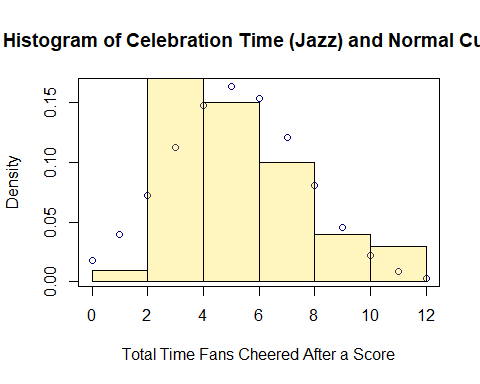
\includegraphics{finalpresentation_files/figure-beamer/unnamed-chunk-12-1.pdf}

\begin{table}
\centering
\begin{tabular}{c|c|c|c|c|c}
\hline
Opposing Team & Year & Game Time & Point \# & Celebration Time & Location\\
\hline
Sporting Kansas City & 2021 & 23:57 & 1 & 35.70 & away\\
\hline
Sporting Kansas City & 2021 & 18:24 & 2 & 43.40 & away\\
\hline
Minnesota United & 2021 & 6:42 & 1 & 24.20 & home\\
\hline
Los Angeles FC & 2018 & 20:31 & 1 & 21.59 & away\\
\hline
Los Angeles FC & 2018 & 9:57 & 2 & 25.64 & away\\
\hline
Los Angeles FC & 2018 & 20:54 & 3 & 38.67 & away\\
\hline
\end{tabular}
\end{table}

Here we have created a histogram of our cheering data for Utah Jazz
fans. We observe this follows close enough to a normal distribution to
perform a t-test. Therefore, we will conduct a t-test with a 95\%
confidence interval to provide good evidence to the range of the
population mean.

Here are some summary statistics for RSL fans' celebration times:

\begin{Shaded}
\begin{Highlighting}[]
\FunctionTok{summary}\NormalTok{(rslCelebrationTimes)}
\end{Highlighting}
\end{Shaded}

\begin{verbatim}
##    Min. 1st Qu.  Median    Mean 3rd Qu.    Max. 
##   13.34   30.17   38.60   41.13   49.19   95.20
\end{verbatim}

\begin{verbatim}
## 
##  One Sample t-test
## 
## data:  jazzCelebrationTimes
## t = 14.828, df = 49, p-value < 2.2e-16
## alternative hypothesis: true mean is not equal to 0
## 95 percent confidence interval:
##  4.41557 5.80003
## sample estimates:
## mean of x 
##    5.1078
\end{verbatim}

From this t-test we have observed with 95\% confidence the population
mean will be within (4.4155696, 5.8000304) seconds. Now we will do this
same analysis on the RSL fan data.

\begin{table}
\centering
\begin{tabular}{c|c|c|c|c|c}
\hline
Opposing Team & Year & Game Time & Point \# & Celebration  Time & Location\\
\hline
Sporting Kansas City & 2021 & 23:57 & 1 & 35.70 & away\\
\hline
Sporting Kansas City & 2021 & 18:24 & 2 & 43.40 & away\\
\hline
Minnesota United & 2021 & 6:42 & 1 & 24.20 & home\\
\hline
Los Angeles FC & 2018 & 20:31 & 1 & 21.59 & away\\
\hline
Los Angeles FC & 2018 & 9:57 & 2 & 25.64 & away\\
\hline
Los Angeles FC & 2018 & 20:54 & 3 & 38.67 & away\\
\hline
\end{tabular}
\end{table}

Just like the Jazz fan data we have tracked variables of opposing team,
year, game time, point number, celebration time, and location. We will
be focusing on the celebration time in this analysis. First we will
calculate mean and standard deviation values. Then we will use these
values to create a normal curve distribution and overlay this with a
histogram from our data.

\includegraphics{finalpresentation_files/figure-beamer/unnamed-chunk-17-1.pdf}

The histogram of our RSL fan data seems to line up decently with a
normal distribution. It is shifted a little to the left and has a couple
outliers on the right side. This is probably due to some factors such as
a game winning goal late into the game. Next, we will conduct a t-test
with a 95\% confidence interval as we have done with the Jazz fan data.

\begin{verbatim}
## 
##  One Sample t-test
## 
## data:  rslCelebrationTimes
## t = 17.62, df = 49, p-value < 2.2e-16
## alternative hypothesis: true mean is not equal to 0
## 95 percent confidence interval:
##  36.4379 45.8197
## sample estimates:
## mean of x 
##   41.1288
\end{verbatim}

From this t-test we have observed with 95\% confidence the population
mean will be within (36.4379047, 45.8196953) seconds.

Next, we will perform a two-variable t-test using a 95\% confidence
level to determine if there is a difference bewtween Jazz fans'
celebration times and RSL fans' celebration times.

\begin{verbatim}
## 
##  Welch Two Sample t-test
## 
## data:  jazzCelebrationTimes and rslCelebrationTimes
## t = -15.266, df = 51.133, p-value < 2.2e-16
## alternative hypothesis: true difference in means is not equal to 0
## 95 percent confidence interval:
##  -40.7577 -31.2843
## sample estimates:
## mean of x mean of y 
##    5.1078   41.1288
\end{verbatim}

As we can see from the previous t-test, we can say with 95\% confidence
that the population means are not equal. The 95\% confidence interval
for this t-test is (-40.7576978, -31.2843022). This confidence interval
says that on average, Jazz fans' celebration time are shorter than RSL
fans' celebration time.
\end{block}
\end{frame}

\begin{frame}{Limitations}
\protect\hypertarget{limitations}{}
As discussed earlier, the data we have gathered is probably not totally
random. However, it is possible that the data we have good is somewhat
good at representing the underlying populations. We tried to get random
data as much as possible, but we ran into issues such as sports games
being unavailable for viewing. To alleviate these problems, we gathered
data from different games. Additionally, our large sample size of 50 for
both Jazz and RSL helped make the data more representative.

There is also the matter of data. All our data come from sports games
which have taken place in the past few years. In the context of our
question, it could be argued that gathering data from a wide range of
years may have been better. However, it is also reasonable to say that
data from recent years is more relevant to most people---sports fans may
not care too much about what happened decades ago, and they may be more
interested in data from recent years.
\end{frame}

\begin{frame}{Conclusion}
\protect\hypertarget{conclusion}{}
\end{frame}

\end{document}
